%!TEX options=--shell-escape
\documentclass[tikz]{standalone}
\usepackage[T1]{fontenc}
\usepackage[utf8]{inputenc}
\usepackage{xcolor}
\usepackage{amsmath}
\usepackage{amssymb}
\usepackage{hyperref}
\usepackage{accsupp}    
\usepackage{graphicx}
\usepackage{mathtools}
\usepackage{pagecolor}
\usepackage{amsmath} % for \dfrac
\usepackage{tikz}
\tikzset{>=latex} % for LaTeX arrow head
\usepackage{braket}
\usepackage{pgfplots} 
\usepackage[edges]{forest}
\usetikzlibrary{patterns, backgrounds, arrows.meta}
\setlength{\parindent}{0cm}
\setlength{\parskip}{1em}

\usetikzlibrary{patterns}

\begin{document}
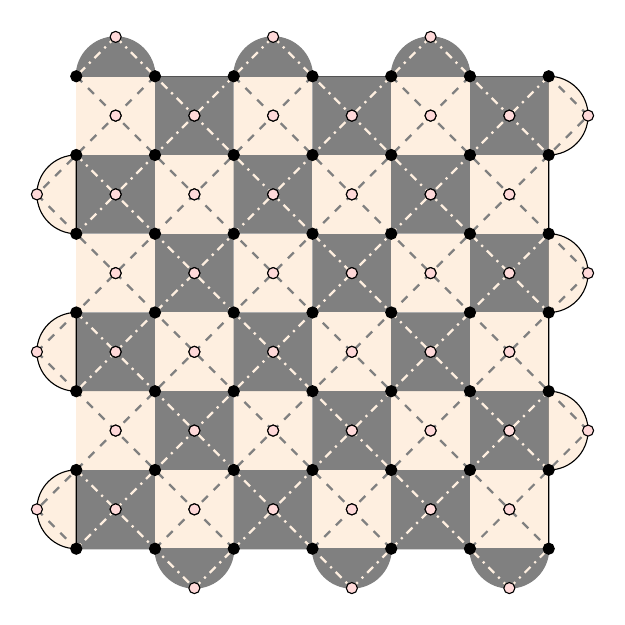
\begin{tikzpicture}[]
   \draw (0, 0) -- (6, 0) -- (6, 6) -- (0, 6) -- cycle;
   \foreach \y in {0,2,...,4}{
    \foreach \x in {0,2,...,4}{
        \fill[gray] (\x,\y) rectangle (1+\x,1+\y) rectangle (2+\x,2+\y);
        \fill[yellow!40!red!10] (\x+1,\y) rectangle (\x+2,\y+1);
        \fill[yellow!40!red!10] (\x,\y+1) rectangle (\x+1,\y+2);
    }}
 \foreach \x in {0, 2,...,4}{
    \draw[gray, fill=gray] (\x,0) -- (1+\x,0) arc (0:180:-0.5) -- cycle;
    \draw[gray, fill=gray](\x,6) -- (1+\x,6) arc (0:180:0.5) -- cycle;
    }
    \foreach \y in {0, 2,...,4}{
    \draw[fill=yellow!40!red!10] (0,\y) -- (0,1+\y) arc (90:270:0.5);
    \draw[fill=yellow!40!red!10] (6,\y) -- (6,1+\y) arc (90:270:-0.5);
    }

    \foreach \x in {0, 1, ...,5}{
        \foreach \y in {0, 1, ...,5}{
            \filldraw[draw=black, fill=pink!60] (\x + 0.5, \y + 0.5) circle[radius=2pt] node[font=\tiny] {};
        }
    }

    % X Lattice
    \foreach \x in {0, 2, ..., 5}{
            \draw[thick, dashed, gray] (\x, 0) -- (0, \x);
            \draw[thick, dashed, gray] (\x, 6) -- (6, \x);
            \draw[thick, dashed, gray] (\x + 1, 6) -- (-0.5, 4.5 - \x);
            \draw[thick, dashed, gray] (\x + 1, 0) -- (6.5, 5.5 - \x);
            \draw[thick, dashed, gray] (-0.5, \x + 0.5) -- (0, \x);
            \draw[thick, dashed, gray] (6.5, \x + 1.5) -- (6, \x + 2);
    }

    % Z Lattice
    \foreach \x in {1, 3, ..., 6}{
            \draw[thick, dash dot, yellow!40!red!10] (0, \x) -- (\x + 0.5, -0.5);
            \draw[thick, dash dot, yellow!40!red!10] (\x - 0.5, 6.5) -- (6, \x);
            \draw[thick, dash dot, yellow!40!red!10] (\x + 1, 6) -- (0, 5 - \x);
            \draw[thick, dash dot, yellow!40!red!10] (\x + 1, 0) -- (6, 5 - \x);
            \draw[thick, dash dot, yellow!40!red!10] (\x + 0.5, -0.5) -- (\x + 1, 0);
            \draw[thick, dash dot, yellow!40!red!10] (\x - 0.5, 6.5) -- (\x - 1 , 6);
    }


    \foreach \x in {0, 1, ...,5}{
        \foreach \y in {0, 1, ...,5}{
            \filldraw[draw=black, fill=pink!60] (\x + 0.5, \y + 0.5) circle[radius=2pt] node[font=\tiny] {};
        }
    }

    \foreach \x in {0, 2, ...,5}{
        \filldraw[draw=black, fill=pink!60] (\x + 1.5, -0.5) circle[radius=2pt] node[font=\tiny] {};
        \filldraw[draw=black, fill=pink!60] (\x + 0.5, 6.5) circle[radius=2pt] node[font=\tiny] {};
        \filldraw[draw=black, fill=pink!60] (-0.5, \x + 0.5) circle[radius=2pt] node[font=\tiny] {};
        \filldraw[draw=black, fill=pink!60] (6.5, \x + 1.5) circle[radius=2pt] node[font=\tiny] {};
    }
    \foreach \x in {0, 1, ...,6}{
        \foreach \y in {0, 1, ...,6}{
            \filldraw[draw=black] (\x, \y) circle[radius=2pt] node[font=\tiny] {};
        }
    }
\end{tikzpicture} 
\end{document}
